\documentclass[a4paper,12pt]{article} 
\usepackage[T2A]{fontenc}			
\usepackage[utf8]{inputenc}			
\usepackage[english,russian]{babel}
\usepackage{float}
\usepackage{amsmath,amsfonts,amssymb,amsthm,mathrsfs,mathtools} 
\usepackage{cancel}
\usepackage{multirow}
\usepackage[colorlinks, linkcolor = blue]{hyperref}
\usepackage{upgreek}\usepackage[left=2cm,right=2cm,top=2cm,bottom=3cm,bindingoffset=0cm]{geometry}
\usepackage{tikz}
\usepackage{graphicx}
\usepackage{subfig}
\usepackage{titletoc}
\usepackage{pgfplots}
\usepackage{xcolor}
\usepackage{wrapfig}
\usepackage{pgfplots}
\pgfplotsset{width=10cm,compat=1.9}

\begin{document}

\begin{titlepage}
		\vspace*{\fill}
		
		\begin{center}
			
\includegraphics[scale=0.8]{MIPT.pdf}
			\\[0.7cm]\Huge Московский Физико-Технический Институт
			\\[2cm]\LARGE Отчет по эксперименту
			\\[0.5cm]\noindent\rule{\textwidth}{1pt}
			\\\Huge\textbf{4.1.1. \\ Изучение центрированных оптических систем}
			\\[-0.5cm]\noindent\rule{\textwidth}{1pt}
		\end{center}
		
		\vspace*{\fill}
		
		\begin{flushleft}
			Выполнила: \hspace{\fill} Группа:
			\\Малиновская София \hspace{\fill} Б05-102
		\end{flushleft}
	\end{titlepage}

	\setcounter{page}{2}


\section*{Цель работы}
Изучение свойств оптических систем: определение фокусных расстояний линз, определение фокусных расстояний и положения главной и фокальной плоскостей сложной оптической системы, изучение аббераций оптических систем.


\section*{В работе используются} 
Оптическая скамья с набором рейтеров, положительные и отрицательные линзы, экран, осветитель с ирисовой диафрагмой, зрительная труба, кольцевые диафргамы, линейка.


\section*{Теоретическая сводка}
\subsection*{Определения фокусных расстояний}
Формула тонкой линзы имеет вид
\begin{equation}
    \frac{1}{f} = \frac{1}{a} + \frac{1}{b},
\end{equation}
\noindent
где $f$ -- фокусное расстояние, $a$ -- расстояния от предмета до линзы, $b$ -- расстояние от изображения до линзы.

\noindent
Для измерения фокусного расстояния тонкой собирающей линзы может использоваться схема с рис. 1. и формула (2).
\begin{equation}
    f = \frac{L^2 - l^2}{4L}
\end{equation}

\begin{figure}[H]
    \centering
    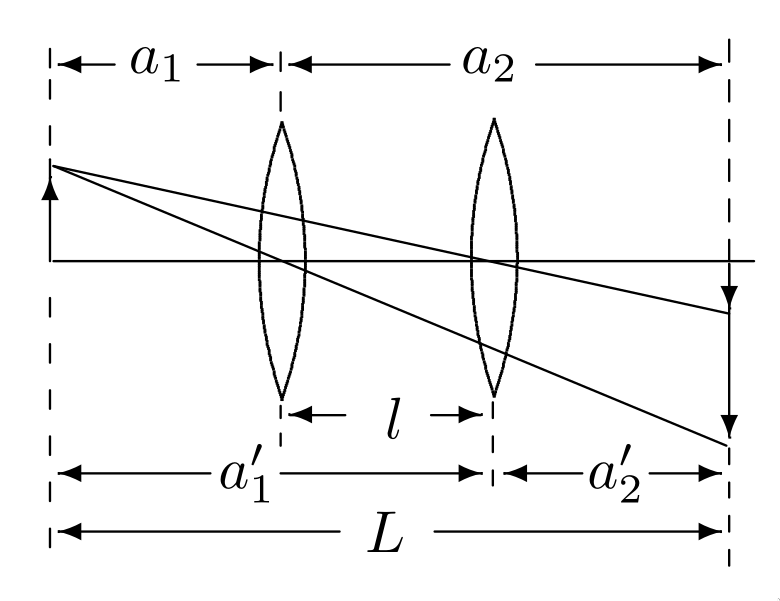
\includegraphics[scale=0.3]{pic_1.png}
    \caption{Схема измерения фокуса тонкой собирающей линзы}
\end{figure}

\noindent
Также фокусное расстояние тонкой собирабщей линзы можно измерить с помощью зрительной трубы, настроенной на бесконечность. Если расположить линзу между предметом и трубой и найти четкое изображение предмета, то расстояние от линзы до предмета будет равно фокусному.

\noindent
Для определения расстояние тонкой рассеивающей линзы поспользуемся схемой на рис. 2 и формулой тонкой линзы. Также можно восползоваться зриетльной трубой, настроенной на бесконечность. Если расположить предмет у нее в фокусе, то изображение переместиться в бесконечность, что можно проверить с помощью зрительной трубы.

\begin{figure}[H]
    \centering
    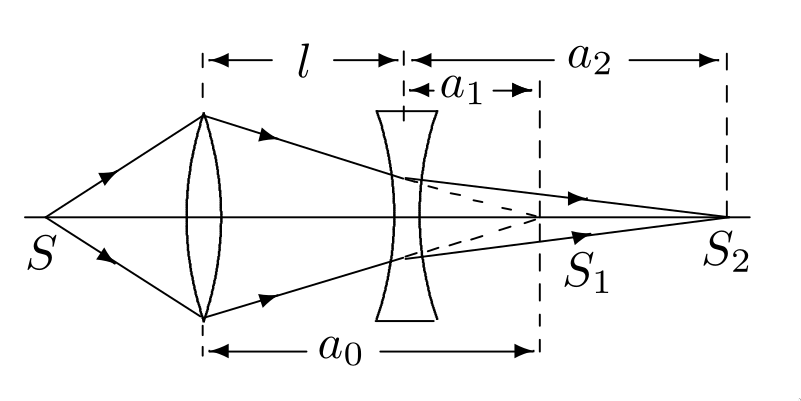
\includegraphics[scale=0.35]{pic_2.png}
    \caption{Схема измерения фокуса тонкой рассеивающей линзы}
\end{figure}

\noindent
Для определения фокусного расстояние и положения главных плоскостей сложной оптической системы может использоваться метод Аббе: схема на рис. 3 и формула (3).

\begin{figure}[H]
    \centering
    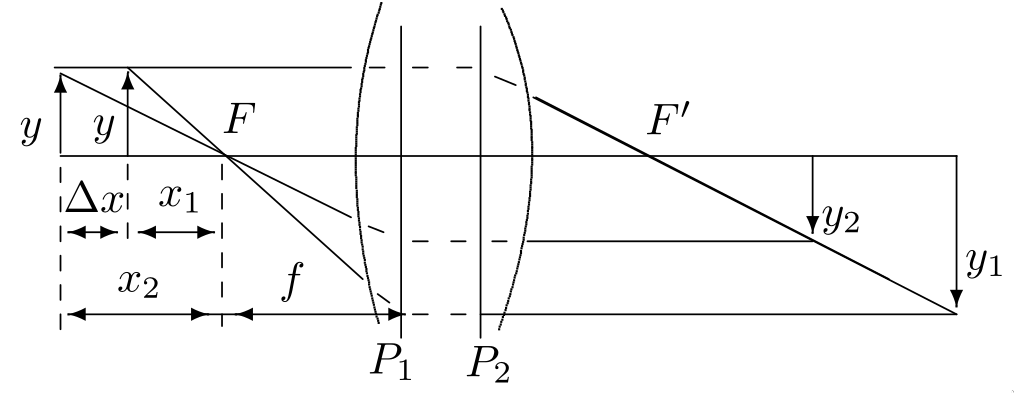
\includegraphics[scale=0.3]{pic_3.png}
    \caption{Схема определения фокусного расстояние и положения главных плоскостей сложной оптической}
\end{figure}

\begin{equation}
    f = \frac{\Delta x}{y / y_1 - y / y_2}    
\end{equation}


\subsection*{Аберрации реальных оптических систем}
Сферическая аберрация -- аберрация, связанная с формой линзы. При прохождении через нее не параксиального пучка лучи, проходящие на разных расстояниях от главной оптической оси собираются в разных точках. Для количечественной оценки сферической аберрации будем пользоваться характеристической кривой сферической аберрации, то есть зависимостью 
\begin{equation}
    \delta s(h) = s(h) - s(0) = -\frac12 \left( \frac{n}{n - 1} \right)^2 \left( \frac{h}{f} \right)^2 f
\end{equation}
\noindent
При $h = r$ формула (4) определяет продольную сферическую аберрацию. \\
Хроматическая аберрация -- аберрация, связанная с немонохроматичностью проходящего через линзу света. Показатель преломления вещества зависит от длины волны падающего света, а значит лучу с разынами длинами волны будут собираться в разных точках. Для количечественной оценки хроматической аберрации воспользуемся соотношениями
\begin{equation}
    \delta f_\text{хр} = f_F - f_C,
\end{equation}
\begin{equation}
    \nu = \frac{n_D - 1}{n_F - n_C},
\end{equation}
\begin{equation}
    \delta f_\text{хр} = -\frac{1}{\nu} f_D,
\end{equation}
\noindent
где $f_F$ -- фоккусное расстояние для длины волны 486.1 нм, $f_C$ -- фокусное расстояние для длины волны 656.3 нм, $f_D$ -- фокусное расстояние для длины волны 589.3 нм, $\nu$ -- число Аббе.


\section*{Ход работы}
\subsection*{Определения фокусных расстояний}
\paragraph{Юстировка} сначала разделим имеющийся набор на собирающие и рассеивающие линзы и отцентрируем установку. Собирающие линзы: 1, 2, 3; рассеивающие линзы: 4.

\paragraph{Определение фокусных расстояний линз с помощью экрана}
Воспользуемся сначала схемой на рис. 1 и формулой (2) для определения фокусного расстояния линзы 1. При измерении расстояний получаем $L = 48.0 \pm 0.2$ см, $l = 25.1 \ pm 0.2$ см. Отсюда ее фокусное расстояние $f = 8.7 \pm 0.3$ см. \\
Также мы можем воспользоваться формулой тонкой линзы для определения фокусного расстояния: $a = 31.0 \pm 0.3$, $b = 14.0 \pm 0.3$. Тогда $f = 10.0 \pm 0.5$ см. \\
Теперь воспользуемся схемой на рис. 2 и формулой тонкой линзы для определения фокусного расстояния рассеивающей линзы 4: $a_0 = 31 \pm 0.3$ см, $l = 24.2 \pm 0.3$ см, $a_2 = 17.5$ см. Отсюда $f = 8.5 \pm 4$ см.

\paragraph{Определение фокусных расстояний линз с помощью зрительной трубы}
Фокусные расстояния, определенные с помощью зрительной трубы, составляют
\begin{itemize}
    \item для линзы 1 $f = 10.5 \pm 0.3$ см, что существенно отличается от значения $f = 8.7 \pm 0.3$ см, полученного ранее, поэтому линзу нельзя считать тонкой.
    \item для линзы 2 $f = 13.4 \pm 0.3$ см.
    \item для линзы 4 $f = 9.0 \pm 0.4$ см.
\end{itemize}

\paragraph{Определение фокусного расстояния сложной оптической системы} воспользуемся схемой на рис. 3 и формулой (3) для определения фокусного расстояния и положения главных плоскостей системы методом Аббе. Для этого сначала соберем установку согласно рис. 3, расположив линзы 1 и 2 на расстоянии  на расстоянии $l_{12} = 30$ см друг от друга. Измерив необходимые расстояния, получаем: $\Delta x = 2.4 \pm 0.3$ см, $y_1 = 5.1 \pm 0.1$ см, $y_2 = 12.3 \pm 0.1$ см, $y = 2.0$ см. Отсюда фокусное расстояние системы $f = 10.5 \pm 0.5$ см. С помощью зрительной трубы найдем главные фокусы системы: для этого закрепим трубу за второй линзой и будем отодвигать источник, пока не увидим четкое изображение. Для определения второго фокуса поменяем линзы местами, не меняя расстояний в системе. Полученные значения главынх фокусов $F_{1\Sigma} = 5.1 \pm 0.3$ см, $F_{2\Sigma} = 4.5 \pm 0.3$ см.

\subsection*{Аберрации реальных оптических систем}
\paragraph{Сферические аберрации} для качетсвенного наблюдения сферических аберраций расположим осветитель и экран на дальних концах скамьи. Линзу 3 расположим на расстоянии чуть большем фокусного от источника. На источник наденем маску минимального размера. Перемещая линзу, получим на экране четкое изображение. При смеге маски наблюдаем, что пр неизменном расстоянии от источника до линзы расстояние от линзы до изображения заметно меняется. Это объясняется сферической аберрацией. \\
Для количественной оценки сферической аберрации сначала получим параллельный пучок от линзы для параксиальных лучей. Затем, увеличиваю диаметр маски, будем менять положение линзы с помощью нониусного винта и измерять расстояния по нониусной шкале $d$. Резульаты измерений представлены в табл. 1. Погрешность измерения $d$ составляет $0.1$ мм.

\begin{table}[H]
    \centering
    \caption{Сферические абберации}
    \begin{tabular}{|c|c|c|c|} \hline
        $h$, мм & 0 & 5 & 20 \\ \hline
        $d$, мм & 0 & 0.8 & 2.9 \\ \hline
    \end{tabular}
\end{table}

\noindent
По результатм этих измерений построим зависимость $\delta s(h)$, представленную на рис. 4. Эксраполируя эту зависимость до $h = r$, где $r$ -- радиус линзы, найдем продольную аберрацию $\delta s(r) = \Delta f(r) = 3.6$ мм.

\begin{figure}[H]
    \centering
    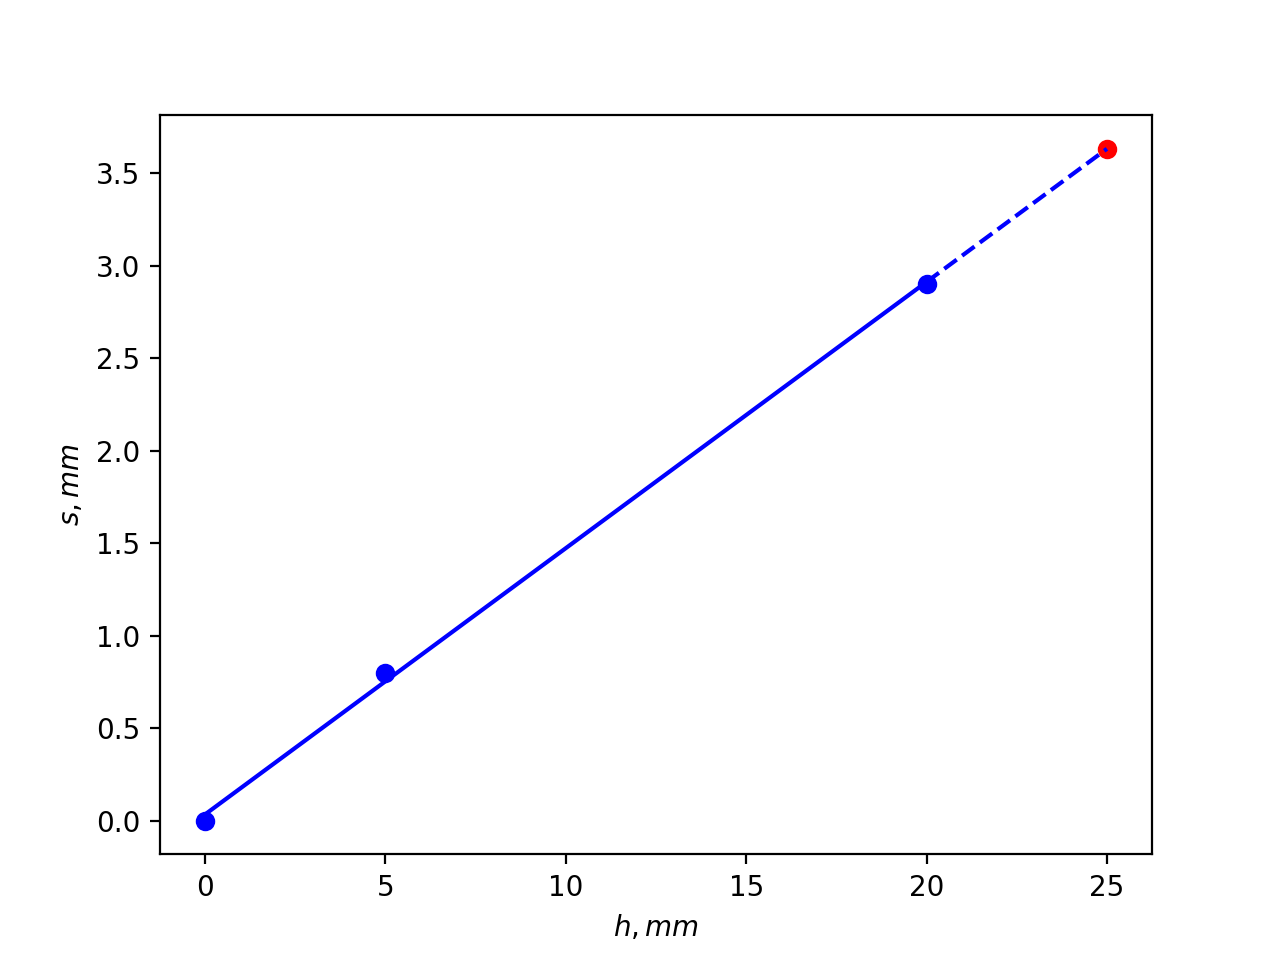
\includegraphics[scale=0.9]{1.png}
    \caption{Сферические аберрации}
\end{figure}

\newpage
\paragraph{Хроматические аберрации} пользуясь тремя светофильтрами, найдем значения $f_D = 13.5$ мм, $f_F = 13.9$ мм, $f_C = 13,3$ мм. Отсюда, пользуясь формулами (5) и (7), находим $\nu \approx 23$, $\delta f_\text{хр} = 0.6$ мм.


\section*{Вывод}
Мы измерили фокусные расстояния нескольких линз, а также системы линз. Получены значения:
\begin{itemize}
    \item для линзы 1 фокусное расстояние $f = 10.5 \pm 0.3$ cм, линзу нельзя считать тонкой
    \item для линзы 2 фокусное расстояние $f = 13.4 \pm 0.3$ см
    \item для линзы 4 фокусное расстояние $f = 9.0 \pm 0.4$ см при измерении с помощью трубы, $f = 8.5 \pm 0.4$ см при измерении с помощью экрана. Линзу можно считать тонкой
    \item для системы из линз 1 и 2 фокусное расстояние состаляет $f = 10.5 \pm 0.5$ см, положения главынх фокусов $F_{1\Sigma} = 5.1 \pm 0.3$ см, $F_{2\Sigma} = 4.5 \pm 0.3$ см
\end{itemize}
Также качественно пронаблюдали и оценили сферические и хроматические абберации. Получены значения продольной сферической аберрации $\delta s(r) = 3.6$ мм и хроматической аберрации $\delta f_\text{хр} = 0.6$ мм, а также оценено число Аббе $\nu \approx 23$.


\end{document}

